\documentclass[12pt,a4paper] {report}

% Packages
\usepackage{graphicx}
\usepackage{amsmath}
\usepackage{hyperref}
\usepackage{setspace}
\usepackage{listings}
\usepackage{xcolor}  % Include xcolor for text color

\lstset{
  literate={\_}{{\_}}{1},   % Replace _ with the literal \_
  basicstyle=\scriptsize\ttfamily,      % Optional: Set typewriter font for listings
  breaklines=true,            % Enable line breaking for long lines
  postbreak=\mbox{\textcolor{red}{$\hookrightarrow$}\space}, % Optional: indicate line break
  literate={|}{{\textbar}}1 {0}{{0}}1 {>}{{\textgreater}}1 {\_}{{\_}}1,
  escapechar=\%             % Optional: Set an escape character if needed
}
% Title and Author (adjust the spacing as needed)
\title{\LARGE \textbf{Quantum Networking: Explore QKD and quantum internet}}
\author{}
\date{\large On: \today}

% Begin Document
\begin{document}

% Title Page
\makeatletter
\begin{titlepage}
\centering
\vspace* {1cm}
{ 
\includegraphics[width=6cm]{ELMEPA.png}}\\[1cm]

{\LARGE \textbf{Quantum Networking: Explore QKD and quantum internet}}\\[1cm]
Project for\\[1cm]

	Advanced Networks Master's program course\\[0.5cm]



	\textbf{Written By:} {Nikolaos Mouzakitis MTP321}\\[1cm]
\date{\large Date Last Edited: \today}
{\@date\\}
\end{titlepage}
\makeatother
% Abstract


	\chapter* {Abstract}
	\addcontentsline{toc} {chapter} {Abstract}

		Quantum networking represents a transformative advancement in secure communication,
		with Quantum Key Distribution (QKD) and the quantum internet standing at its core.
		Unlike the widely available and adopted classical systems, QKD leverages certain mechanical principles
		from the field of quantum physics in order to theoretically guarantee unbreakable encryption schemes,
		addressing critical vulnerabilities in modern cryptographic methods.
		In the early days of its rise, quantum internet promises a global network enabling unprecedented levels of
		secure communication, distributed quantum computing, and advanced scientific applications.

% Table of Contents
\tableofcontents

        % Chapters
        \chapter{Introduction}

		Quantum networking stands as the next frontier in communication technology,
		which is expected to leverage principles of quantum mechanics for
		achieving unprecedented levels in security, as well as in computational capability.
		In contrast to ordinary classical networks, quantum networks rely on quantum states
		of the likes of superposition and entanglement to achieve operations impossible for
	        the classic networking schemes. These attributes become of vital importance in 
		application areas like secure communications, where quantum key distribution (QKD) 
		promises provable security against eavesdropping, and in distributed computing in cases 
		where quantum nodes could collaborate to solve problems beyond the reach of classical networks.
		In the modern world, where the requirement for global data security keeps following
		an increasing trend, quantum networking is considered as a robust solution
		for protecting sensitive informations.
		Moreover, it is possible that mixed architectures combining classical and quantum network elements
		could provide a feasible solution for the future communication systems.

			              %#############################################
		Challenges arise although; despite the promising potential in quantum networking,
		it faces technical and theoretical obstacles that need to be surpassed
		in order to achieve and enable an entirely practical implementation and adoption.
		Because of the very nature of quantum mechanichs, quantum internet is opted to utilize concepts
		without classical counterparts with the likes of quantum entanglment,
		no-cloning theorem, quantum measurement and teleportation.
%1		
		In contrast to the classical and well known model of computation experienced so far,
		where we deeply rely on the fact that information can be read and copied, this concept that does not hold
		for quantum networking. 
%2		
		The scalability remains one of the main issues,
		because as current quantum networks are limited in the number of nodes and the
		distances they can span without degradation.
		This limitation comes from the fragile nature of the quantum states,
		which are very sensitive on environmental noise and decoherence especially over long distances.
		As a countermeassure, in order to avoid these limitations the development of reliable quantum repeaters
		and advanced error-correction schemes are required. 

		Additionally, the efficient generation, distribution and storage of entanglement 
		across a network pose critical hurdles, as maintaining high fidelity in entangled
		states is necessary for the network's functionality.
%3	        
		Another key challenge lies in integrating
	        quantum systems with classical infrastructure,
	        which requires seamless coordination between
	        vastly different operational paradigms.
	        Addressing these challenges is crucial for moving quantum
		networking beyond the experimental
		phase and into real-world applications.
		The computing power of a quantum computer is exponentialy
		related to the number of qubits that comprise it;
		where a qubit is the quantum counterpart of the classical bit and is the building block of a quantum computers.

		In this project the current state of quantum networking is explored alongside its potential applications. 
		The introduction provides a broad overview of the field, emphasizing its importance in secure communication and distributed computing. 
		In the related work section recent advancements in quantum networking are presented, with a focusing on technologies such as 
		quantum key distribution, entanglement distribution, and quantum repeaters. 
		In the methodology section, a simulation-based approach utilizing QuTiP showcases examples to study the key elements of quantum networking. 
		The results section presents findings from the simulations, 
		highlighting performance metrics such as communication fidelity and error rates under varying network conditions. 
		The discussion section interprets these findings in the context of existing literature, identifying both strengths and limitations of current technologies. 
		In the end, the conclusion section summarizes the project's work.

	\chapter{Related Work}
		In recent years, quantum networking has gained
		significant attention due to its potential to ignite a revolution in
		secure communications and distributed computing.
		Khristo et al. \cite{Khristo2020} have provided an overview of the field's
		current status but also of the desired future directions.
		In their work the key advancements and challenges in the
		development of quantum networks have been discussed while in addition
		explored the integration of the quantum key distribution (QKD)
		and a broader vision for the quantum internet.


	\chapter{Methodology and Results}
		
		For the purposes of this project, a
		simulation approach using software tools
		have been employed in order to enable the
		demonstration of selected concepts in quantum networking.
		QuTiP(Quantum Toolbox in Python)\cite{qutip}, an open source framework
		written in Python, has been used for the simulations.

		\section{BB84 Quantum Key Distribution Protocol}

		BB84 protocol is a foundational work in the field
		of quantum key distribution (QKD) protocols,
		been proposed back in 1984 \cite{bb84}.
		It realizes a secure communication of a secret cryptographic key
		alongside two entities, over a potenitally insecure medium/channel
		by using principles of quantum mechanics.
		
		In this simulation (code is listed in Listing 1 of Appendix A),
		two entities entitled Alice and Bob, execute the QDK using the BB84 protocol
		in order to share a secret key over a potentially non-secure medium. Initially Alice creates
		a number of qubits (100 in this example) randomly in one of the two possible bases (either 'x' or 'z') and sends them 
		to Bob. Bob on his side, randomly selects a base per qubit and measures it. In the next step, 
		they are comparing their used bases over a classical communication channel and 
		they discard all the bits generated as an outcome from the measured qubits whose bases were not matching.
		The remaining bits which obtained from matching bases among the two entities are kept and create the shared secret key.

		\begin{figure}[h!]
			\centering
			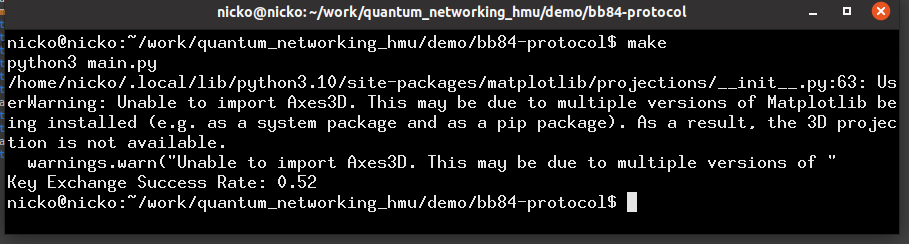
\includegraphics[width=0.8\textwidth]{bb84/success_rate_terminal.png}
			\caption{Execution of code of Listing 1 of Appendix A.}
			\label{fig:}
		\end{figure}		

		\begin{figure}[h!]
			\centering
			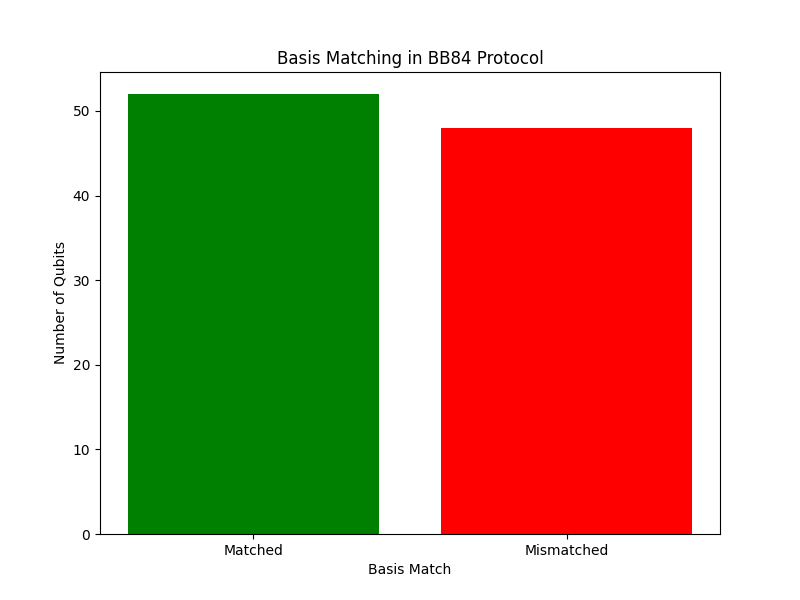
\includegraphics[width=0.4\textwidth]{bb84/basis_matching.png}
			\caption{Bases matched on the example where 100 qubits used.}
			\label{fig:}
		\end{figure}		


		\begin{figure}[h!]
			\centering
			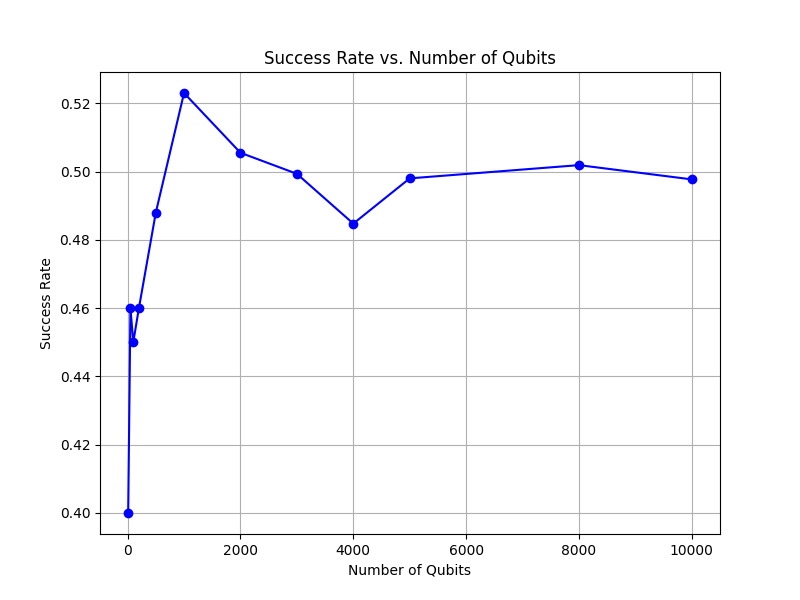
\includegraphics[width=0.5\textwidth]{bb84/success_rate_vs_num_qubits.png}
			\caption{Success rate vs number of qubits used.}
			\label{fig:}
		\end{figure}		
	

		As we can observe in Figure 3.3, the relation of success rate is plotted against the utilized 
		number of qubits in the protocol. The simulation was run for up to 10000 qubits. 
		Success rate is converging to value 0.5, as the probability 
		of Alice and Bob choosing the same base ('x' or 'z') is 50\%.

	\chapter{Discussion}

	\chapter{Conclusion}



\bibliographystyle{plain}
\bibliography{references}
\appendix

\section*{Appendix A: BB84 Quantum Key Distribution Simulation Code}

%\begin{lstlisting}[language=Python, caption=BB84 for QKD, label=code:QKD, escapeinside=||]
\begin{lstlisting}[language=Python, caption=BB84 for QKD, label=code:QKD]
from qutip import basis, ket2dm
import numpy as np
zero = basis(2, 0)  ''' |0> '''
one = basis(2, 1)   ''' |1> ''' 
plus = (zero + one).unit()  ''' |+> '''
minus = (zero - one).unit() ''' |-> ''' 
''' Alice's qubits'''
def generate_bb84_states(num_qubits):
    states = []
    bases = []
    for _ in range(num_qubits):
        basis_choice = np.random.choice(['z', 'x'])
        bit = np.random.choice([0, 1])
        if basis_choice == 'z':
            states.append(zero if bit == 0 else one)
        else:
            states.append(plus if bit == 0 else minus)
        bases.append(basis_choice)
    return states, bases
'''Measurement'''
def measure_state(state, basis):
    if basis == 'z':
        projection = [zero, one]
    else:  ''' 'x' '''
        projection = [plus, minus]
    probabilities = [abs(proj.overlap(state))**2 for proj in projection]
    return np.random.choice([0, 1], p=probabilities)
'''Simulation'''
num_qubits = 100
alice_states, alice_bases = generate_bb84_states(num_qubits)
bob_bases = np.random.choice(['z', 'x'], num_qubits)
''' Measure and compare '''
bob_results = [measure_state(state, bob_bases[i]) for i, state in enumerate(alice_states)]
matching_bases = [alice_bases[i] == bob_bases[i] for i in range(num_qubits)]
shared_key = [bob_results[i] for i in range(num_qubits) if matching_bases[i]]
''' Calculate success rate'''
success_rate = len(shared_key) / num_qubits
print(f"Key Exchange Success Rate: {success\_rate:.2f}")
import matplotlib.pyplot as plt
''' Visualization 1: Basis Matching (Bar Chart)'''
matched = sum(matching_bases)
mismatched = num_qubits - matched
plt.figure(figsize=(8, 6))
plt.bar(['Matched', 'Mismatched'], [matched, mismatched], color=['green', 'red'])
plt.title('Basis Matching in BB84 Protocol')
plt.xlabel('Basis Match')
plt.ylabel('Number of Qubits')
plt.savefig('Basis Matching in BB84 Protocol.png')
''' Visualization 2: Success Rate vs. Number of Qubits (Line Chart) '''
num_qubits_list = [10, 50, 100, 200, 500, 1000, 2000, 3000, 4000, 5000, 8000, 10000]
success_rates = []
for nq in num_qubits_list:
    alice_states, alice_bases = generate_bb84_states(nq)
    bob_bases = np.random.choice(['z', 'x'], nq)
    bob_results = [measure_state(state, bob_bases[i]) for i, state in enumerate(alice_states)]
    matching_bases = [alice_bases[i] == bob_bases[i] for i in range(nq)]
    shared_key = [bob_results[i] for i in range(nq) if matching_bases[i]]
    success_rate = len(shared_key) / nq
    success_rates.append(success_rate)
plt.figure(figsize=(8, 6))
plt.plot(num_qubits_list, success_rates, marker='o', color='b')
plt.title('Success Rate vs. Number of Qubits')
plt.xlabel('Number of Qubits')
plt.ylabel('Success Rate')
plt.grid(True)
plt.savefig("Success Rate vs Number of Qubits.png")

\end{lstlisting}
\end{document}
